\documentclass[12pt,a4paper]{article}
\usepackage[utf8]{inputenc}
\usepackage[english]{babel}
\usepackage{amsmath}
\usepackage{amsfonts}
\usepackage{amssymb}
\usepackage{graphicx}
\usepackage{lmodern}
\usepackage[left=3cm,right=2cm,top=2cm,bottom=2cm]{geometry}

\usepackage{tikz}
	\usetikzlibrary{calc}
	\usetikzlibrary{shapes}
	\usetikzlibrary{arrows}
	\usetikzlibrary{fit}

\usepackage[section]{placeins}
\usepackage{here}

\title{Interaction-Agents}
\author{Julien Gori}
\begin{document}
\maketitle

\newpage

\tableofcontents

\newpage

\section{Introduction}

Interaction-Agents is a Python module destined to help design intelligent user interfaces (IUI). It does so in two ways:
\begin{itemize}
\item It proposes an interaction model, in which most IUIs can be described. This allows a standardization in the interaction model description. Tasks, user models and interface models can be bundled together into a so-called \emph{Bundle}. This facilitates re-use of models among researchers; in particular it makes comparing different solutions much easier.
\item It facilitates implementation, evaluation and comparisons by providing various wrappers around \emph{Bundles}, to e.g.
	\begin{itemize}
	\item Evaluate user and interface models,
	\item Train a user model for a given interface,
	\item Find the best (train) interface given a user model,
	\item Jointly train interface and user models,
	\item Combine several bundles to perform different subtasks.
	\end{itemize}
\end{itemize}

\section{Overview of the Interaction Model}
\subsection{Notations}
\begin{itemize}
\item $s_T$: state of the task
\item $s_O$: internal state of the operator
\item $s_A$: internal state of the assistant

\end{itemize}
\subsection{Operator-Assistant Model}
The operator-assistant model is represented Fig.~\ref{fig:opass}. The model assumes two agents, the operator and the assistant, and a task. The operator is assumed to want to drive the task to a certain state $s_T$, and the assistant is here to help the operator achieve its goal.
In the traditional language of user interfaces, the operator is the user, while the assistant is the intelligent tool/interface.


\begin{figure}[H]
\centering
\resizebox{.8\textwidth}{!}{
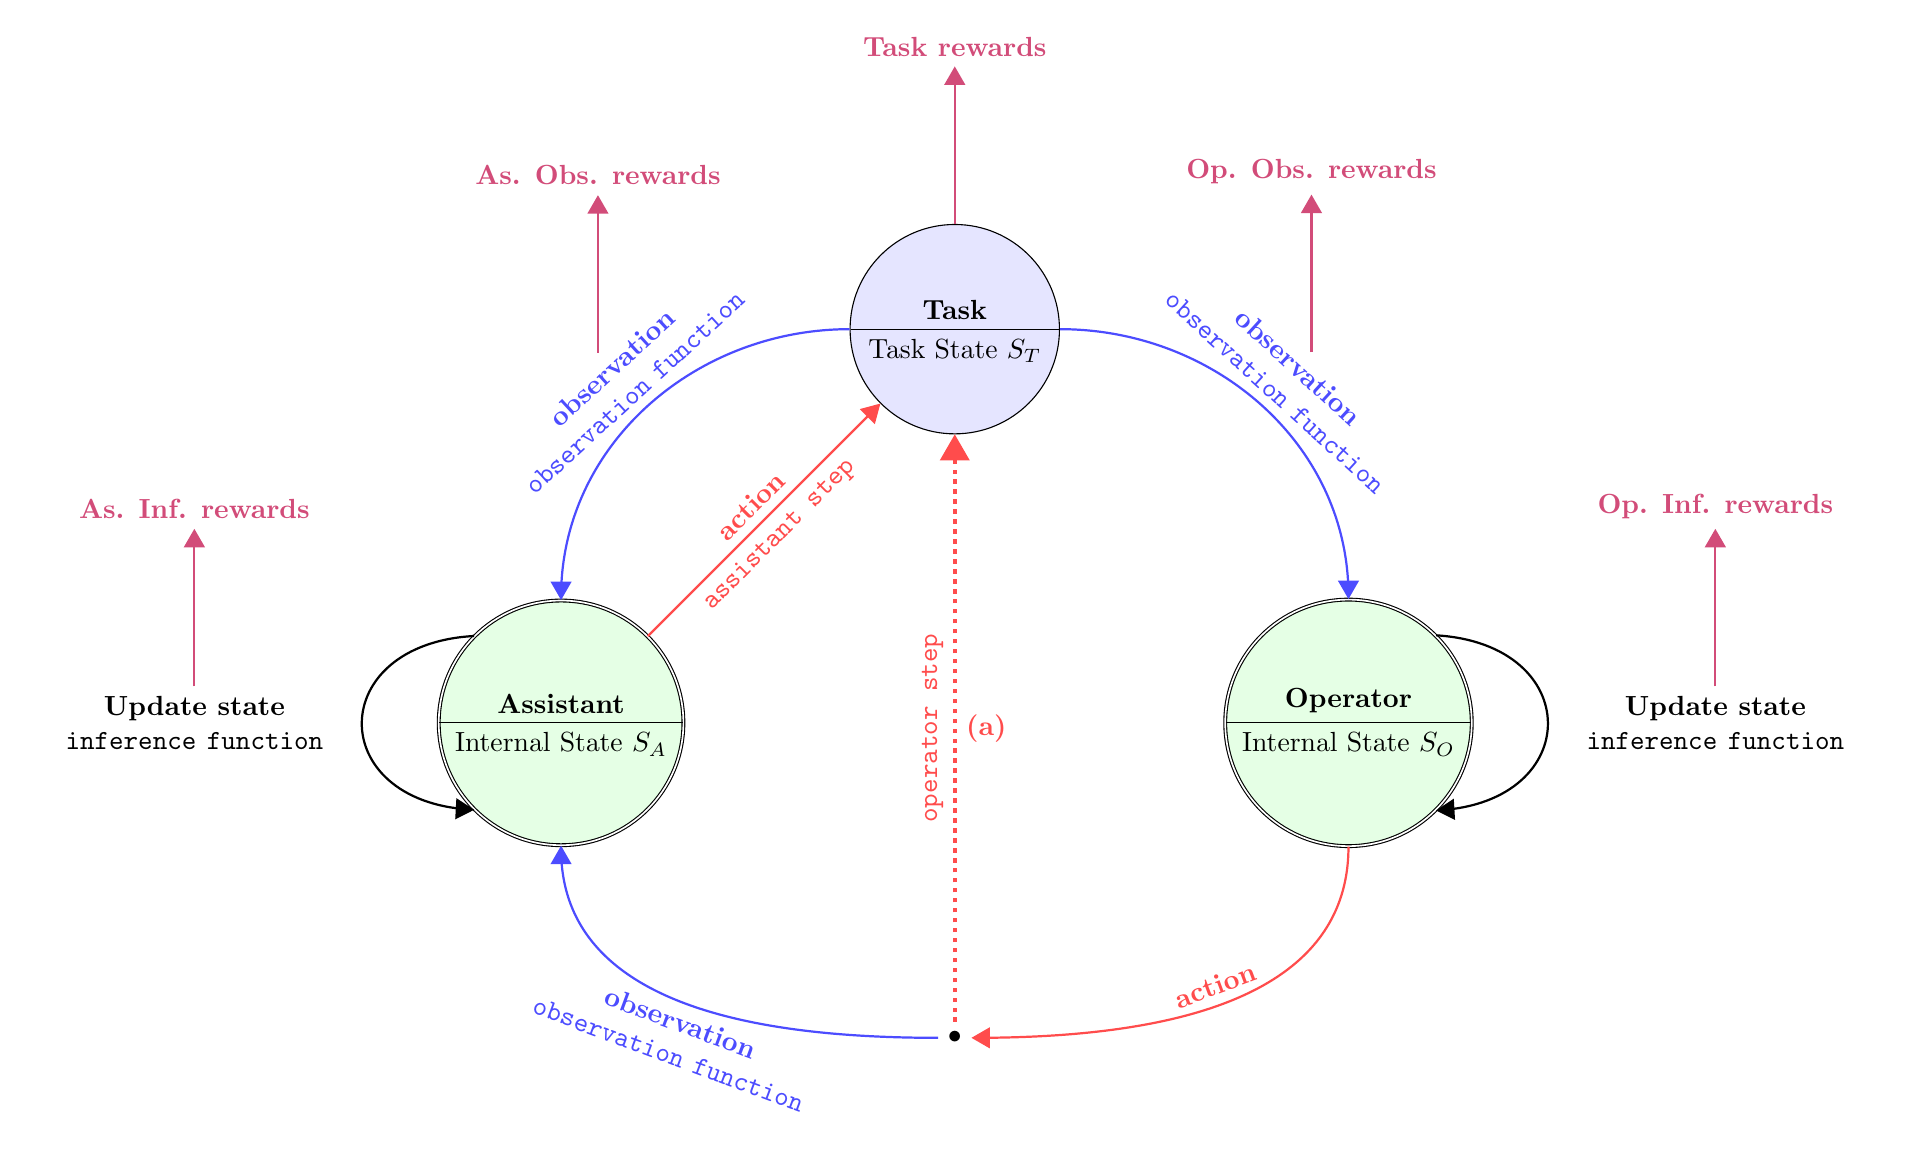
\begin{tikzpicture}
	\tikzstyle{every text node part}=[font=\bfseries]
	\tikzset{agent/.style = {circle split, draw, double, fill = green!10}}

%% Task node

\draw (0,0) node[name = task, circle split, draw, fill = blue!10]{Task \nodepart{lower}{Task State $S_T$}};
	
%% Operator Node
\draw (5,-5) node[agent, name = operator]{
	Operator
	\nodepart{lower}{Internal State $S_O$}	
	};
	
%% Invis node
\draw (0,-9) node[name = null]{$\bullet$};

	
%% assistant Node
\draw (-5,-5) node[agent, name = assistant]{
	Assistant
	\nodepart{lower}{Internal State $S_A$}	
	};
	
%% Edges
\draw[-triangle 60, thick, blue!70] (task.0) to[out = 0, in = 90] node[midway, sloped, above, text width = 4cm, text centered](label1){observation \texttt{observation~function}}(operator.90);

\draw[thick, -triangle 60, red!70] (operator.270) to[out = 270, in = 0] node[midway, sloped, above]{action} (null.0);
\draw[-triangle 60, dotted, ultra thick, red!70] (null) -- node[midway, right]{(a)} node[midway, rotate = 90, above]{\texttt{operator step}} (task.270);
\draw[-triangle 60, thick, blue!70] (null) to[out = 180, in = 270] node[midway, sloped, below, text width = 4cm, text centered](label3){observation \texttt{observation~function}} (assistant.270);
\draw[-triangle 60, thick, blue!70] (task.180) to[out = 180, in = 90] node[midway, sloped, above, text width = 4cm, text centered](label4){observation \texttt{observation~function}} (assistant.90);
\draw[-triangle 60, thick, red!70] (assistant.45) -- node[midway, above, sloped]{action} node[midway, below, sloped]{\texttt{assistant step}} (task.225);
\draw[-triangle 60, thick] (operator.45) .. controls (8,-4) and (8,-6).. node[midway, right, text width = 4cm, text centered](label2){Update state \texttt{inference~function}} (operator.315);
\draw[-triangle 60, thick] (assistant.135) .. controls (-8,-4) and (-8,-6).. node[midway, left, text width = 4cm, text centered](label5){Update state \texttt{inference~function}} (assistant.225);

\draw[-triangle 60, thick, purple!70] (task.90) -- +(0,2) node[above]{Task rewards};
\draw[-triangle 60, thick, purple!70] (label1.90) -- +(0,2) node[above]{Op. Obs. rewards};
\draw[-triangle 60, thick, purple!70] (label2.90) -- +(0,2) node[above]{Op. Inf. rewards};
\draw[-triangle 60, thick, purple!70] (label4.90) -- +(0,2) node[above]{As. Obs. rewards};
\draw[-triangle 60, thick, purple!70] (label5.90) -- +(0,2) node[above]{As. Inf. rewards};
\end{tikzpicture}
}
\caption{Operator-Assistant Model. The presence of the edge labeled (a), i.e. whether or not the operator actions will directly influence the task state, conditions the type of assistance: in case it exists, we will talk of proactive assistance; if not we will talk of supervisory assistance.\label{fig:opass}}
\end{figure}

Agents possess an internal state. Agents can also make \emph{observations} about the task, their internal state, and the other agent's action. Based on these observations, agents can update their internal state using an \emph{inference} process. Agents can also take actions, which may make the state of the task and the agents evolve.



\subsection{State Transition and Observation Probability}
The agents act sequentially; we arbitrarily decide that the operator acts first.
A round of interaction consists of the following transitions, where the superscript $k$ indicates the turn of interaction (a round is played in four turns $0$ --- $3$):
\begin{align}
s^{(0)} \rightarrow o'_O \rightarrow s^{(1)} \rightarrow a'_O \rightarrow s^{(2)} \rightarrow o'_A \rightarrow s^{(3)} \rightarrow a'_A \rightarrow s^{'(0)}.
\end{align}
\noindent For different turns, we define the following joint states:
\begin{align}
s^{(0)} = (0, s_T, s_O, s_A), \\
s^{(1)} = (1, s_T, s'_O, s_A), \\
s^{(2)} = (2, s'_T, s'_O, s_A), \\
s^{(3)} = (3, s'_T, s'_O, s'_A), \\
s^{'(0)} = (0, s''_T, s'_O, s'_A), 
\end{align}
observations:
\begin{align}
o^{(1)} = (o'_O, \text{No-Op}),\\
o^{(2)} = (\text{No-Op}, \text{No-Op}),\\
o^{(3)} = (\text{No-Op}, o'_A),\\
o^{'(0)} = (\text{No-Op}, \text{No-Op}),
\end{align}
and actions:
\begin{align}
a^{(0)} = (\text{No-Op}, \text{No-Op}),\\
a^{(1)} = (a'_O, \text{No-Op}),\\
a^{(2)} = (\text{No-Op}, \text{No-Op}),\\
a^{(3)} =  (\text{No-Op}, a'_A).
\end{align}

We can then see that the operator-assistant model is a Partially Observable Stochastic Game (POSG), with transition and observation probabilities:
\begin{align}
p(s^{(1)}, o^{(1)} | s^{(0)}, a^{(0)}) & = p(o^{(1)} | s^{(0)}, a^{(0)}) \cdot{} p(s^{(1)}| o^{(1)}, s^{(0)}, a^{(0)}) \\
 &= \underbrace{p(o'_O | s^{(0)})}_\text{operator observation function      }  \underbrace{p(s^{(1)}| o'_O, s^{(0)})}_\text{        operator inference function} \\
 p(s^{(2)}, o^{(2)} | s^{(1)}, a^{(1)}) & = p(s^{(2)}| s^{(1)}, a^{(1)}) \\
 &= \underbrace{p(s^{(2)}| s^{(1)}, a'_O)}_\text{        operator step function} \\
 p(s^{(3)}, o^{(3)} | s^{(2)}, a^{(2)}) & = p(o^{(3)} | s^{(2)}, a^{(2)}) \cdot{} p(s^{(3)}| o^{(3)}, s^{(2)}, a^{(2)}) \\
 &= \underbrace{p(o'_A | s^{(2)})}_\text{assistant observation function      }  \underbrace{p(s^{(3)}| o'_A, s^{(2)})}_\text{        assistant inference function} \\
 p(s^{'(0)}, o^{'(0)} | s^{(3)}, a^{(3)}) & = p(s^{'(0)}| s^{(3)}, a^{(3)}) \\
 &= \underbrace{p(s^{'(0)}| s^{(3)}, a'_A)}_\text{        assistant step function} \\
\end{align}
\subsection{Components of the Operator-Assistant Model}


\begin{figure}
\centering
\resizebox{.5\textwidth}{!}{
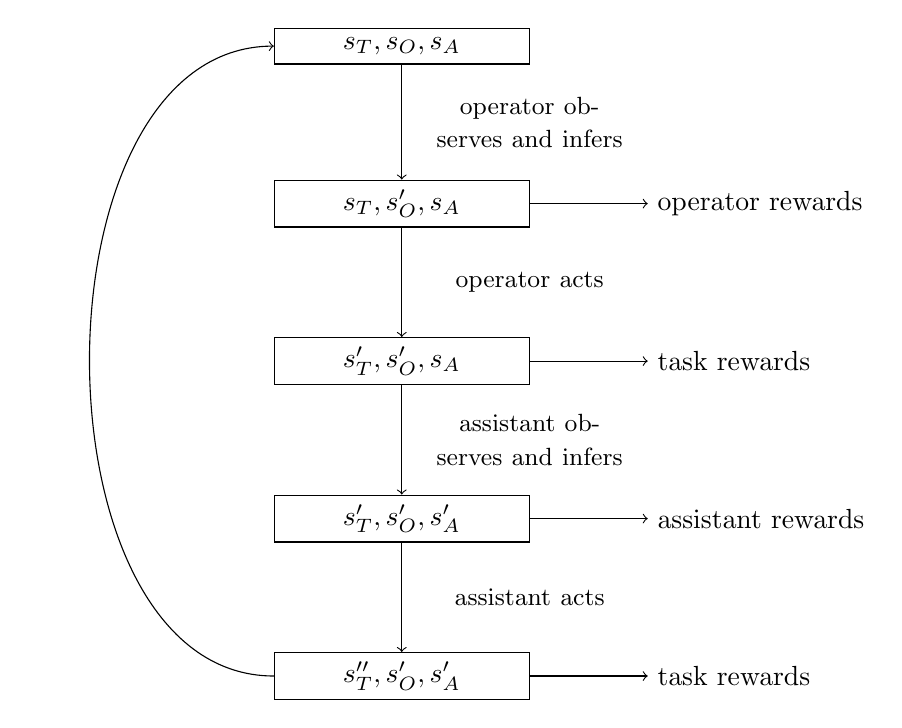
\begin{tikzpicture}
\draw (0,0) node[rectangle, draw = black, name = s0, text width = 3cm, text centered]{$s_T, s_O, s_A$};
\draw (s0) + (0,-2) node[rectangle, draw = black, name = s1, text width = 3cm, text centered]{$s_T, s'_O, s_A$};
\draw[->] (s0) -- node[midway, right, text width = 3cm, text centered]{\small operator observes and infers} (s1);
\draw[->] (s1.0) -- + (1.5,0) node[right]{operator rewards};
\draw (s1) + (0,-2) node[rectangle, draw = black, name = s2, text width = 3cm, text centered]{$s'_T, s'_O, s_A$};
\draw[->] (s1) -- node[midway, right, text width = 3cm, text centered]{\small operator acts} (s2);
\draw[->] (s2.0) -- + (1.5,0) node[right]{task rewards};
\draw (s2) + (0,-2) node[rectangle, draw = black, name = s3, text width = 3cm, text centered]{$s'_T, s'_O, s'_A$};
\draw[->] (s2) -- node[midway, right, text width = 3cm, text centered]{\small assistant observes and infers} (s3);
\draw[->] (s3.0) -- + (1.5,0) node[right]{assistant rewards};
\draw (s3) + (0,-2) node[rectangle, draw = black, name = s4, text width = 3cm, text centered]{$s''_T, s'_O, s'_A$};
\draw[->] (s3) -- node[midway, right, text width = 3cm, text centered]{\small assistant acts} (s4);
\draw[->] (s4.0) -- + (1.5,0) node[right]{task rewards};
\draw[->] (s4.180) to[out=180, in=180] (s0.180);
\end{tikzpicture}
}
\caption{Order of operations in the operator-assistant model}
\end{figure}
 
Explanation of the components of the operator-assistant model:
\begin{itemize}
\item Operator observers: Operator observes (parts of) the task state, as well as inspects its own state.
\item Operator infers: Based on its observation, the operator infers its new state. For example, they might update an internal model that is maintained, e.g. to model the environment or the opponent.
\item Observation and inferring might incur costs. Observation might be costly if it requires acquiring information that is hard to find e.g. finding some item with important significance that changed position. Inferring might also incur a mental effort cost. For now I have no intention to actually model this, but let's keep this in mind.
\item Operator acts: Based on its new state, the operator will select an action.
\item Assistant side: Idem, except that the observation and inference costs are likely null (albeit that inference might be costly in terms of computational power).
\end{itemize}


\subsection{Bundles}

The task, operator and assistant are bundled together to form a ``finished'' environment. A bundle has a state \verb bundle.game_state  which is the joint state $s = (0, s_T, s_O, s_A)$.  Several bundles exist:
\begin{itemize}
\item \verb PlayNone , which does not take any action as input. It puts together two agents together at play to perform the task. This allows one to evaluate agents with policies provided.
\item \verb PlayOperator , which takes the operator action as input. It puts together an assistant with defined policy, and an operator without policy. This allows evaluating a policy on line.
\item \verb PlayAssistant , which is the counterpart to the previous bundle with operators and assistants switched.
\item \verb PlayBoth , were the action is the joint (operator, assistant) action. This allows evaluating policies for both agents on-line.
\item \verb SinglePlayOperator , which does not take an assistant as input. It it useful when one wants to develop a pure user model using \emph{interaction-agents}, where the policy is evaluated on-line (similar to \verb PlayOperator )
\item \verb SinglePlayOperatorAuto  is the same as the previous bundle but where the policy is provided to the agent.
\end{itemize}

\begin{figure}
\centering
\makebox[\textwidth]{
\resizebox{1.2\textwidth}{!}{

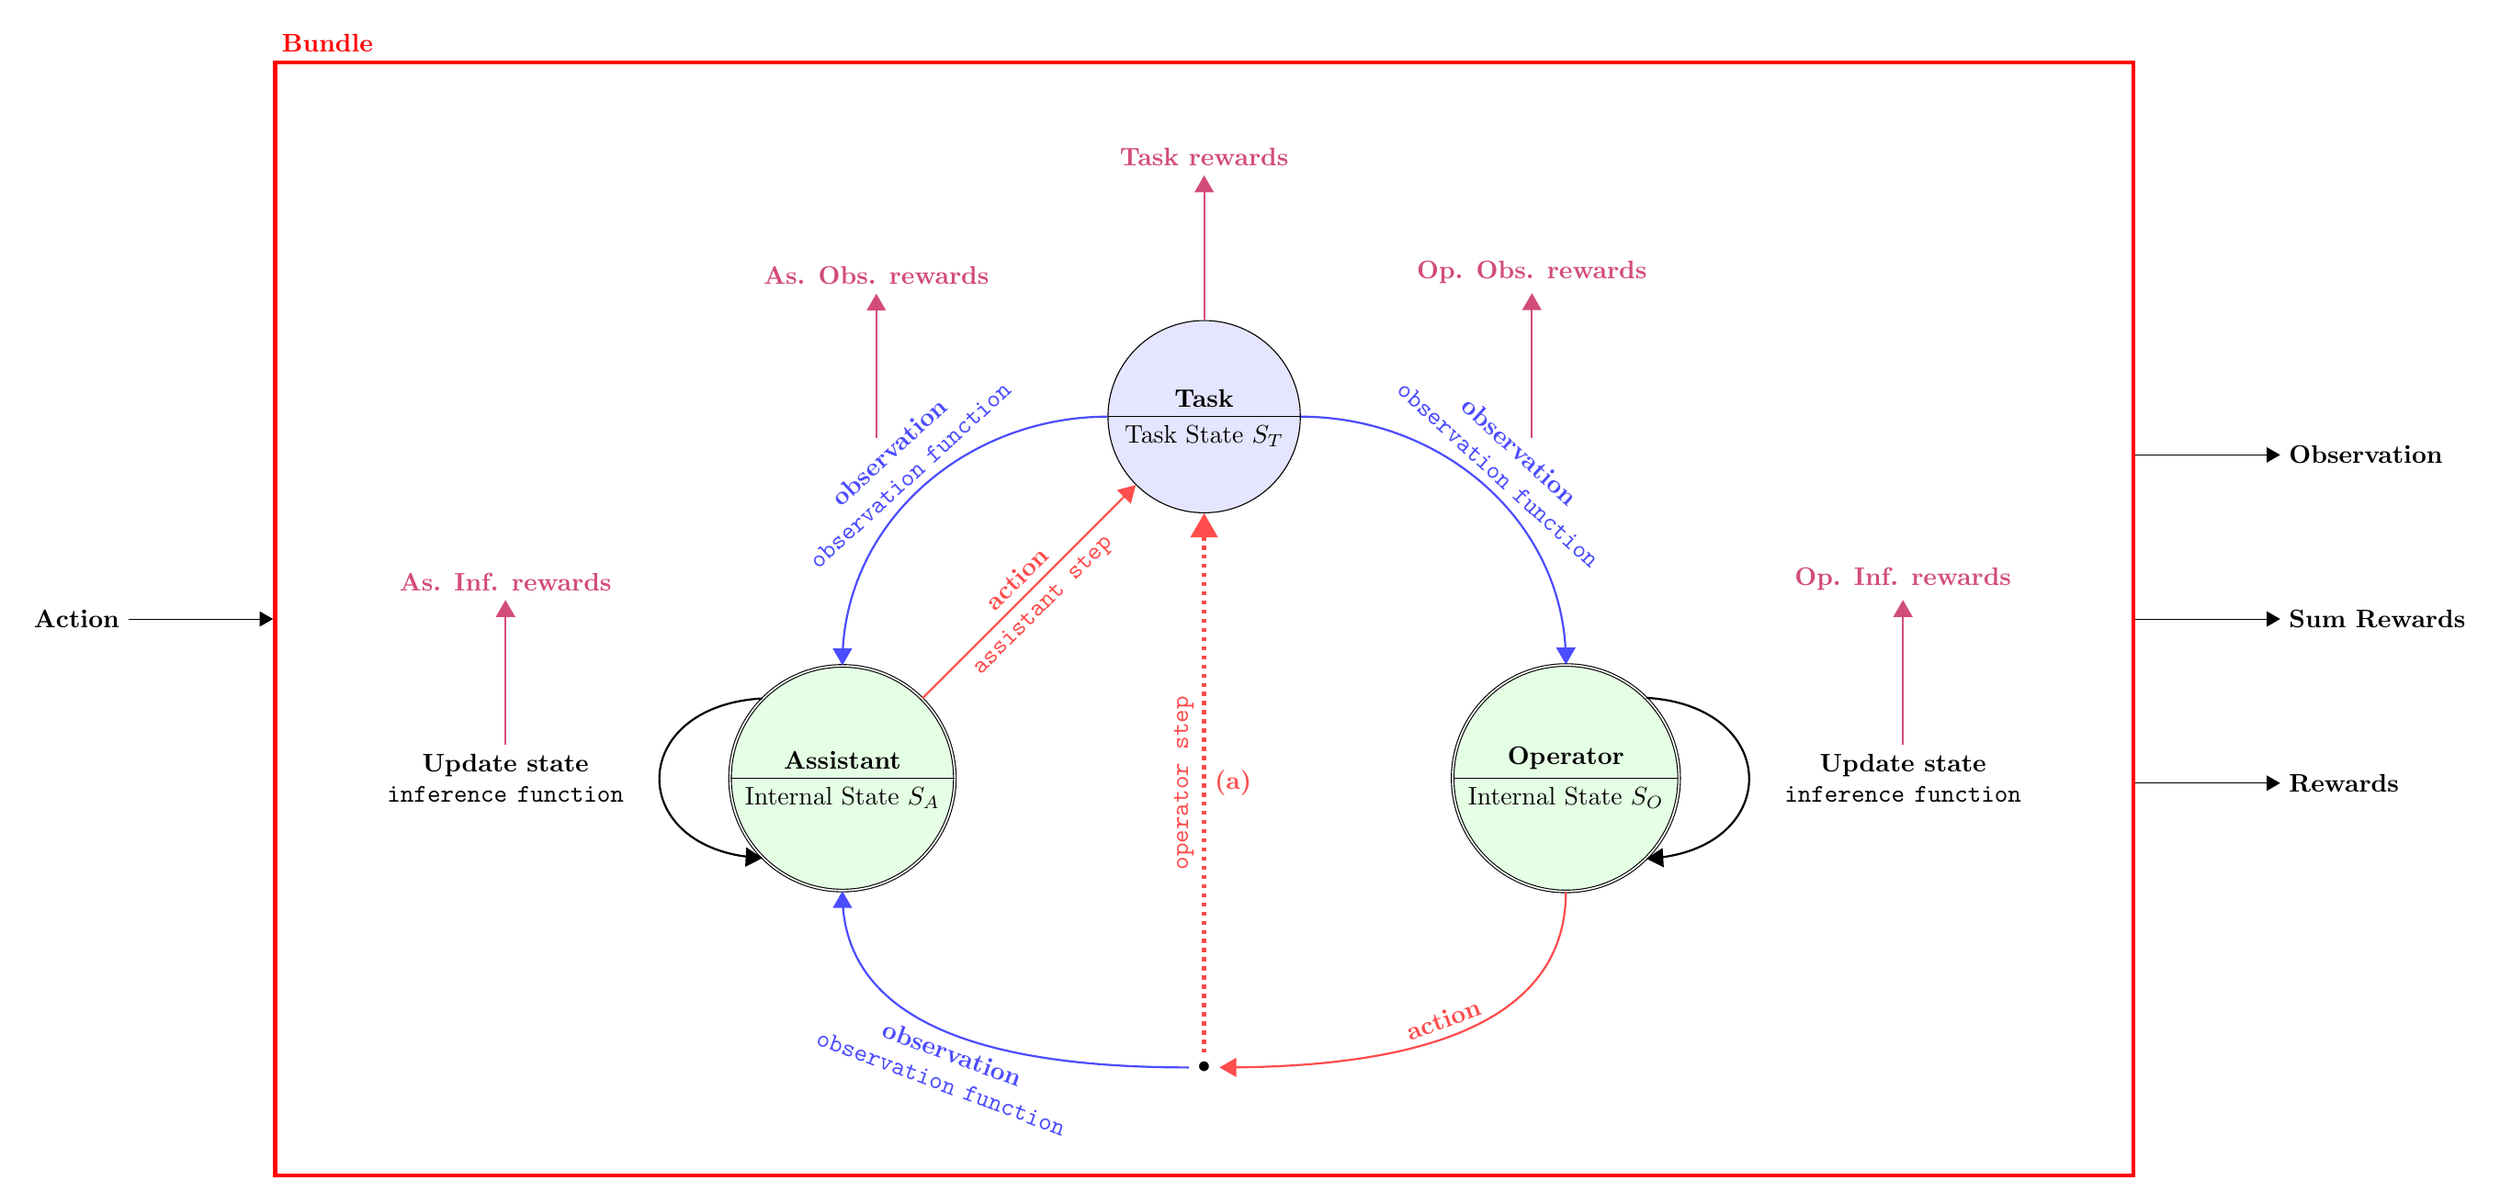
\begin{tikzpicture}
	\tikzstyle{every text node part}=[font=\bfseries]
	\tikzset{agent/.style = {circle split, draw, double, fill = green!10}}

%% Task node

\draw (0,0) node[name = task, circle split, draw, fill = blue!10]{Task \nodepart{lower}{Task State $S_T$}};
	
%% Operator Node
\draw (5,-5) node[agent, name = operator]{
	Operator
	\nodepart{lower}{Internal State $S_O$}	
	};
	
%% Invis node
\draw (0,-9) node[name = null]{$\bullet$};

	
%% assistant Node
\draw (-5,-5) node[agent, name = assistant]{
	Assistant
	\nodepart{lower}{Internal State $S_A$}	
	};
	
%% Edges
\draw[-triangle 60, thick, blue!70] (task.0) to[out = 0, in = 90] node[midway, sloped, above, text width = 4cm, text centered](label1){observation \texttt{observation~function}}(operator.90);

\draw[thick, -triangle 60, red!70] (operator.270) to[out = 270, in = 0] node[midway, sloped, above]{action} (null.0);
\draw[-triangle 60, dotted, ultra thick, red!70] (null) -- node[midway, right]{(a)} node[midway, rotate = 90, above]{\texttt{operator step}} (task.270);
\draw[-triangle 60, thick, blue!70] (null) to[out = 180, in = 270] node[midway, sloped, below, text width = 4cm, text centered](label3){observation \texttt{observation~function}} (assistant.270);
\draw[-triangle 60, thick, blue!70] (task.180) to[out = 180, in = 90] node[midway, sloped, above, text width = 4cm, text centered](label4){observation \texttt{observation~function}} (assistant.90);
\draw[-triangle 60, thick, red!70] (assistant.45) -- node[midway, above, sloped]{action} node[midway, below, sloped]{\texttt{assistant step}} (task.225);
\draw[-triangle 60, thick] (operator.45) .. controls (8,-4) and (8,-6).. node[midway, right, text width = 4cm, text centered](label2){Update state \texttt{inference~function}} (operator.315);
\draw[-triangle 60, thick] (assistant.135) .. controls (-8,-4) and (-8,-6).. node[midway, left, text width = 4cm, text centered](label5){Update state \texttt{inference~function}} (assistant.225);

\draw[-triangle 60, thick, purple!70] (task.90) -- +(0,2) node[name = tasklabel, above]{Task rewards};
\draw[-triangle 60, thick, purple!70] (label1.90) -- +(0,2) node[above]{Op. Obs. rewards};
\draw[-triangle 60, thick, purple!70] (label2.90) -- +(0,2) node[above]{Op. Inf. rewards};
\draw[-triangle 60, thick, purple!70] (label4.90) -- +(0,2) node[above]{As. Obs. rewards};
\draw[-triangle 60, thick, purple!70] (label5.90) -- +(0,2) node[above]{As. Inf. rewards};

\node[draw=red, ultra thick, inner sep = 30pt, fit=(label5.180) (label2.0) (tasklabel.north) (label3.south)](fit) {};
\draw (fit.north west) node[above right, color = red]{Bundle};
\draw[-triangle 60] ($(fit.west) + (-2,0)$) node[left]{Action} -- (fit.west);
\draw[-triangle 60] (fit.10) -- ++ (2,0) node[right]{Observation};
\draw[-triangle 60] (fit.350) -- ++ (2,0) node[right]{Rewards};
\draw[-triangle 60] (fit.east) -- ++ (2,0) node[right]{Sum Rewards};

\end{tikzpicture}
}
}
\caption{Bundle. A task, an operator, and an assistant can be bundled together. The bundle takes as input a joint action and outputs a joint observation, the sum of rewards, as well as each individual reward.\label{fig:bundle}}
\end{figure}

The bundle keeps all states synchronized and handles joint rendering of agents and tasks.



\section{Agents}
\subsection{Overview}
An agent is a combination of 4 components:
	\begin{itemize}
		\item An internal state, which is used to store parameters that belong to the agent and that are susceptible of being updated by the agent,
		\item A policy, which describes what the possible actions of the agents are, and how the agent chooses them.
		\item An observation engine, which produces observations for the agent, from the \verb bundle.game_state .
		\item An inference engine, which uses observations to update the agent's internal state.
	\end{itemize}

An agent can be defined by subclassing the \verb BaseAgent  class.

\begin{figure}
\centering
\resizebox{.8\textwidth}{!}{
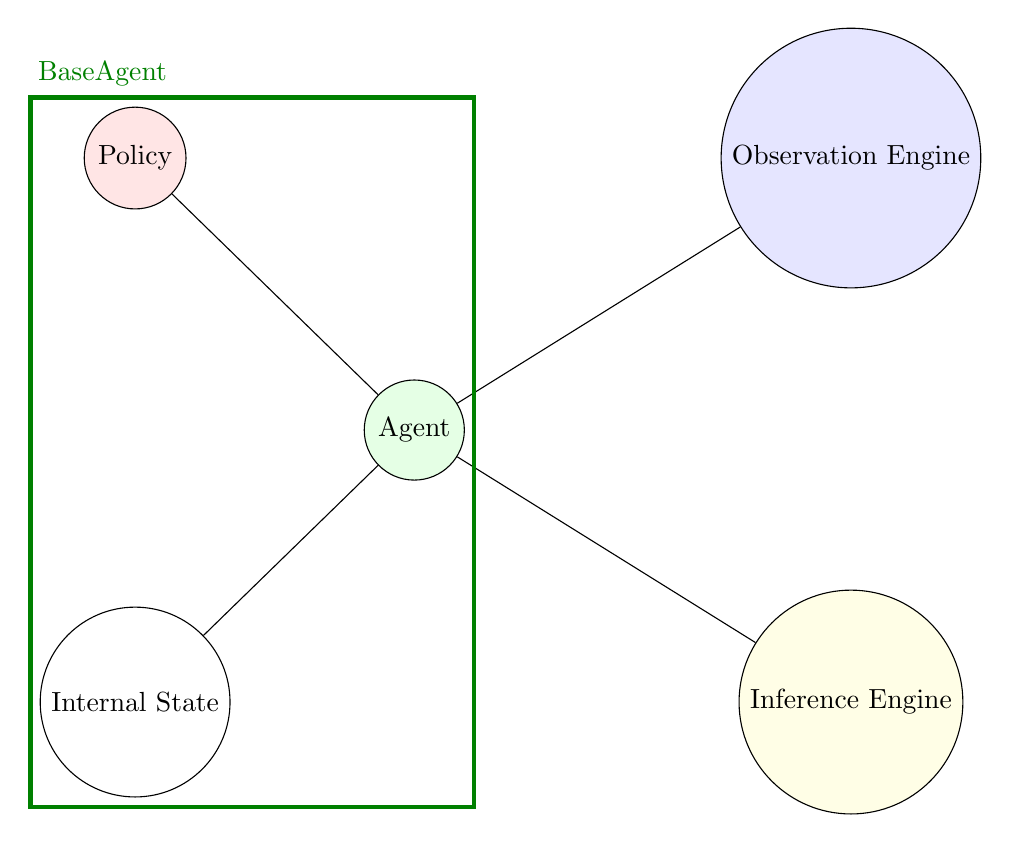
\begin{tikzpicture}
\draw (0,0) node[name = agent, circle, draw = black, fill = green!10!white]{Agent};
\draw (agent.north west) + (6,3) node[name = obs, circle, draw = black, fill = blue!10!white]{Observation Engine};
\draw (agent.south west) + (6,-3) node[name = inf, circle, draw = black, fill = yellow!10!white]{Inference Engine};
\draw (agent.south east) + (-4,-3) node[name = state, circle, draw = black]{Internal State};
\draw (agent.north east) + (-4,3) node[name = pol, circle, draw = black, fill = red!10!white]{Policy};

\draw (agent) -- (obs);
\draw (agent) -- (inf);
\draw (agent) -- (pol);
\draw (agent) -- (state);

\node[draw=green!50!black, ultra thick, fit=(pol.north) (agent.east) (state.south) (state.west)](fit) {};
\draw (fit.north west) node[above right, color = green!50!black]{BaseAgent};

\end{tikzpicture}
}
\caption{An agent is a combination of an observation engine, an inference engine, an internal state and a policy.}
\end{figure}

\subsection{BaseAgent Class}
The \verb BaseAgent  class is the lowest level agent class available in \emph{interaction-agents}. A new agent can be obtained by subclassing the \verb BaseAgent (note that other higher-level agents are already provided by the module, and that it may be faster to subclass such a higher-level agent).




\end{document}